\section{\label{s:system}Transformācijas sistēma}

Šī nodaļa piedāvā uzbūves principus sistēmai, kura ļaus lietotājam dinamiski paplašināt programmēšanas valodas iespējas ar makro valodas palīdzību. Šī makro valoda ļaus izveidot jaunas valodas konstrukcijas no jau eksistējošām vienībām. Sistēma ir projektēta ka virsbūve parsētājam un strādās paralēli ar parsētāju, analizējot kodu ar ierakstītiem makro un apstrādājot daļiņu virknes.

Šīs sistēmas mērķis ir piedāvāt iespēju modificēt valodas sintaksi programmas rakstīšanas gaitā, nebojājot jau eksistējošo konstrukciju darbu. Sistēma ieviesīs pašmodificēšanos lietojot konstrukciju aizvietošanu, kas vienlaikus nodrošinās gramatikas modifikācijas un sākotnējās valodas gramatikas nemainīgumu. Tajā pašā laikā sistēma būs stabila pret kļūdām dēļ tā, ka tā strādās tikai konkrētās gramatikas produkcijas ietvaros un tā, ka tā pārbaudīs tipus jaunizveidotām virknēm.

Sistēmas raksturīga īpašība ir tas, ka tā nav piesaistīta konkrētai programmēšanas valodai. Uz doto brīdi tā var tikt pielāgota un integrēta dažādu valodu parsētājos, kuru arhitektūra atbilst dažiem nosacījumiem. Tai nav ierobežojumu pret atbalstāmo sintaksi, jo tā strādās ārpus valodas gramatikas.

Tālāk nodaļa ir organizēta sekojoši. Apakšnodaļa~\ref{sbs:sys_architecture} iedod ieskatu plānotā sistēmas arhitektūrā. Apakšnodaļa~\ref{sbs:sys_approach} vispārīgi pamato izvēlēto transformācijas pieeju. Apakšnodaļa~\ref{sbs:sys_parserqualities} apraksta īpašības, kuram jāpiemīt parsētājam, lai tas varētu iekļaut transformācijas sistēmu. Apakšnodaļa~\ref{sbs:sys_macrosyntax} apraksta un pamato sistēmas makro sintaksi. Apakšnodaļa~\ref{sbs:sys_qualities} detalizētāk apskata sistēmas sadalījumu uz trim apakšsistēmām un apraksta to sadarbību.

\subsection{\label{sbs:sys_architecture}Sistēmas arhitektūra}

\subsubsection{Makro ielasīšanas soļi}
%Makro ielasīšanas process sastāv no $4$ soļiem, kas notiek secīgi. Sistēmas darbam ir nepieciešama sadarbība ar parsētāju un attiecīga parsētāja saskarne. 

\begin{enumerate}
\item
Parsētājs atpazīst makro sākšanos un izsauc transformācijas sistēmu.
\item
Transformācijas sistēma ielasa makro.
\item
Tipu apakšsistēma pārbauda makro tipu korektumu. Ja tipi ir korekti, turpina uz soli~\ref{i:read_ok}. Ja ielasītā makro tipi nav korekti, turpina uz soli~\ref{i:read_notok}
\item \label{i:read_ok}
Transformācijas sistēma saglabā makro priekš specifiskas produkcijas, lai tālāk apstrādāt programmu.
\item \label{i:read_notok}
Transformācijas sistēma parāda kļūdas paziņojumu par to, ka ielasītā makro tips nesakrīt ar iezīmēto tipu.
\end{enumerate}

\subsubsection{Makro atpazīšanas soļi}

\begin{enumerate}
\item
Parsētājs ienāk kādā no produkciju atpazīšanas funkcijām un izsauc transformācijas sistēmu.
\item
Ja transformācijas sistēmā eksistē makro priekš dotas produkcijas, tā sāk makro atpazīšanas procesu ar soli~\ref{i:match_start}. Citādi tā nedara neko un parsētājs turpina darbu ar soli~\ref{i:match_notok}.
\begin{enumerate}
\item \label{i:match_start}
Transformāciju sistēma pārbauda, vai tajā vietā daļiņu virknē, uz kuru rāda parsētājs, ir sekvence no daļiņām, kas atbilst kādam no makro šabloniem. Ja šāda sekvence eksistē, turpina uz soli~\ref{i:match_ok}. Ja šādas sekvences nav, turpina uz soli~\ref{i:match_notok}.
\item \label{i:match_ok}
Ielasītā sekvence tiek transformēta attiecīgi makro likumam.
\item
Ielasītā sekvence daļiņu virknē tiek aizvietota ar transformēto sekvenci un parsētāja pozīcija tiek uzstādīta uz aizvietotās virknes sākumu. Transformācijas sistēma sāk darbu atkal no soļa~\ref{i:match_start}.
\end{enumerate}
\item \label{i:match_notok}
Parsētājs atjauno darbu no tās pašas vietas daļiņu virknē un sāk gramatikas produkcijas atpazīšanu. %Ja produkcija ir atpazīta, parsētājs turpina darbu no soļa~\ref{i:match_first} ar nākamo produkciju. Ja produkcija nav atpazīta un daļiņu virkne ir beigusies, parsētājs apstājas. Ja produkcija nav atpazīta, parsētājs parāda kļūdas paziņojumu.
\end{enumerate}

Attēls~\ref{fig:match_algorithm} parāda transformācijas sistēmas palaišanu un darbību virkni diagrammas veidā.

\begin{figure}[h!]
  \centering
    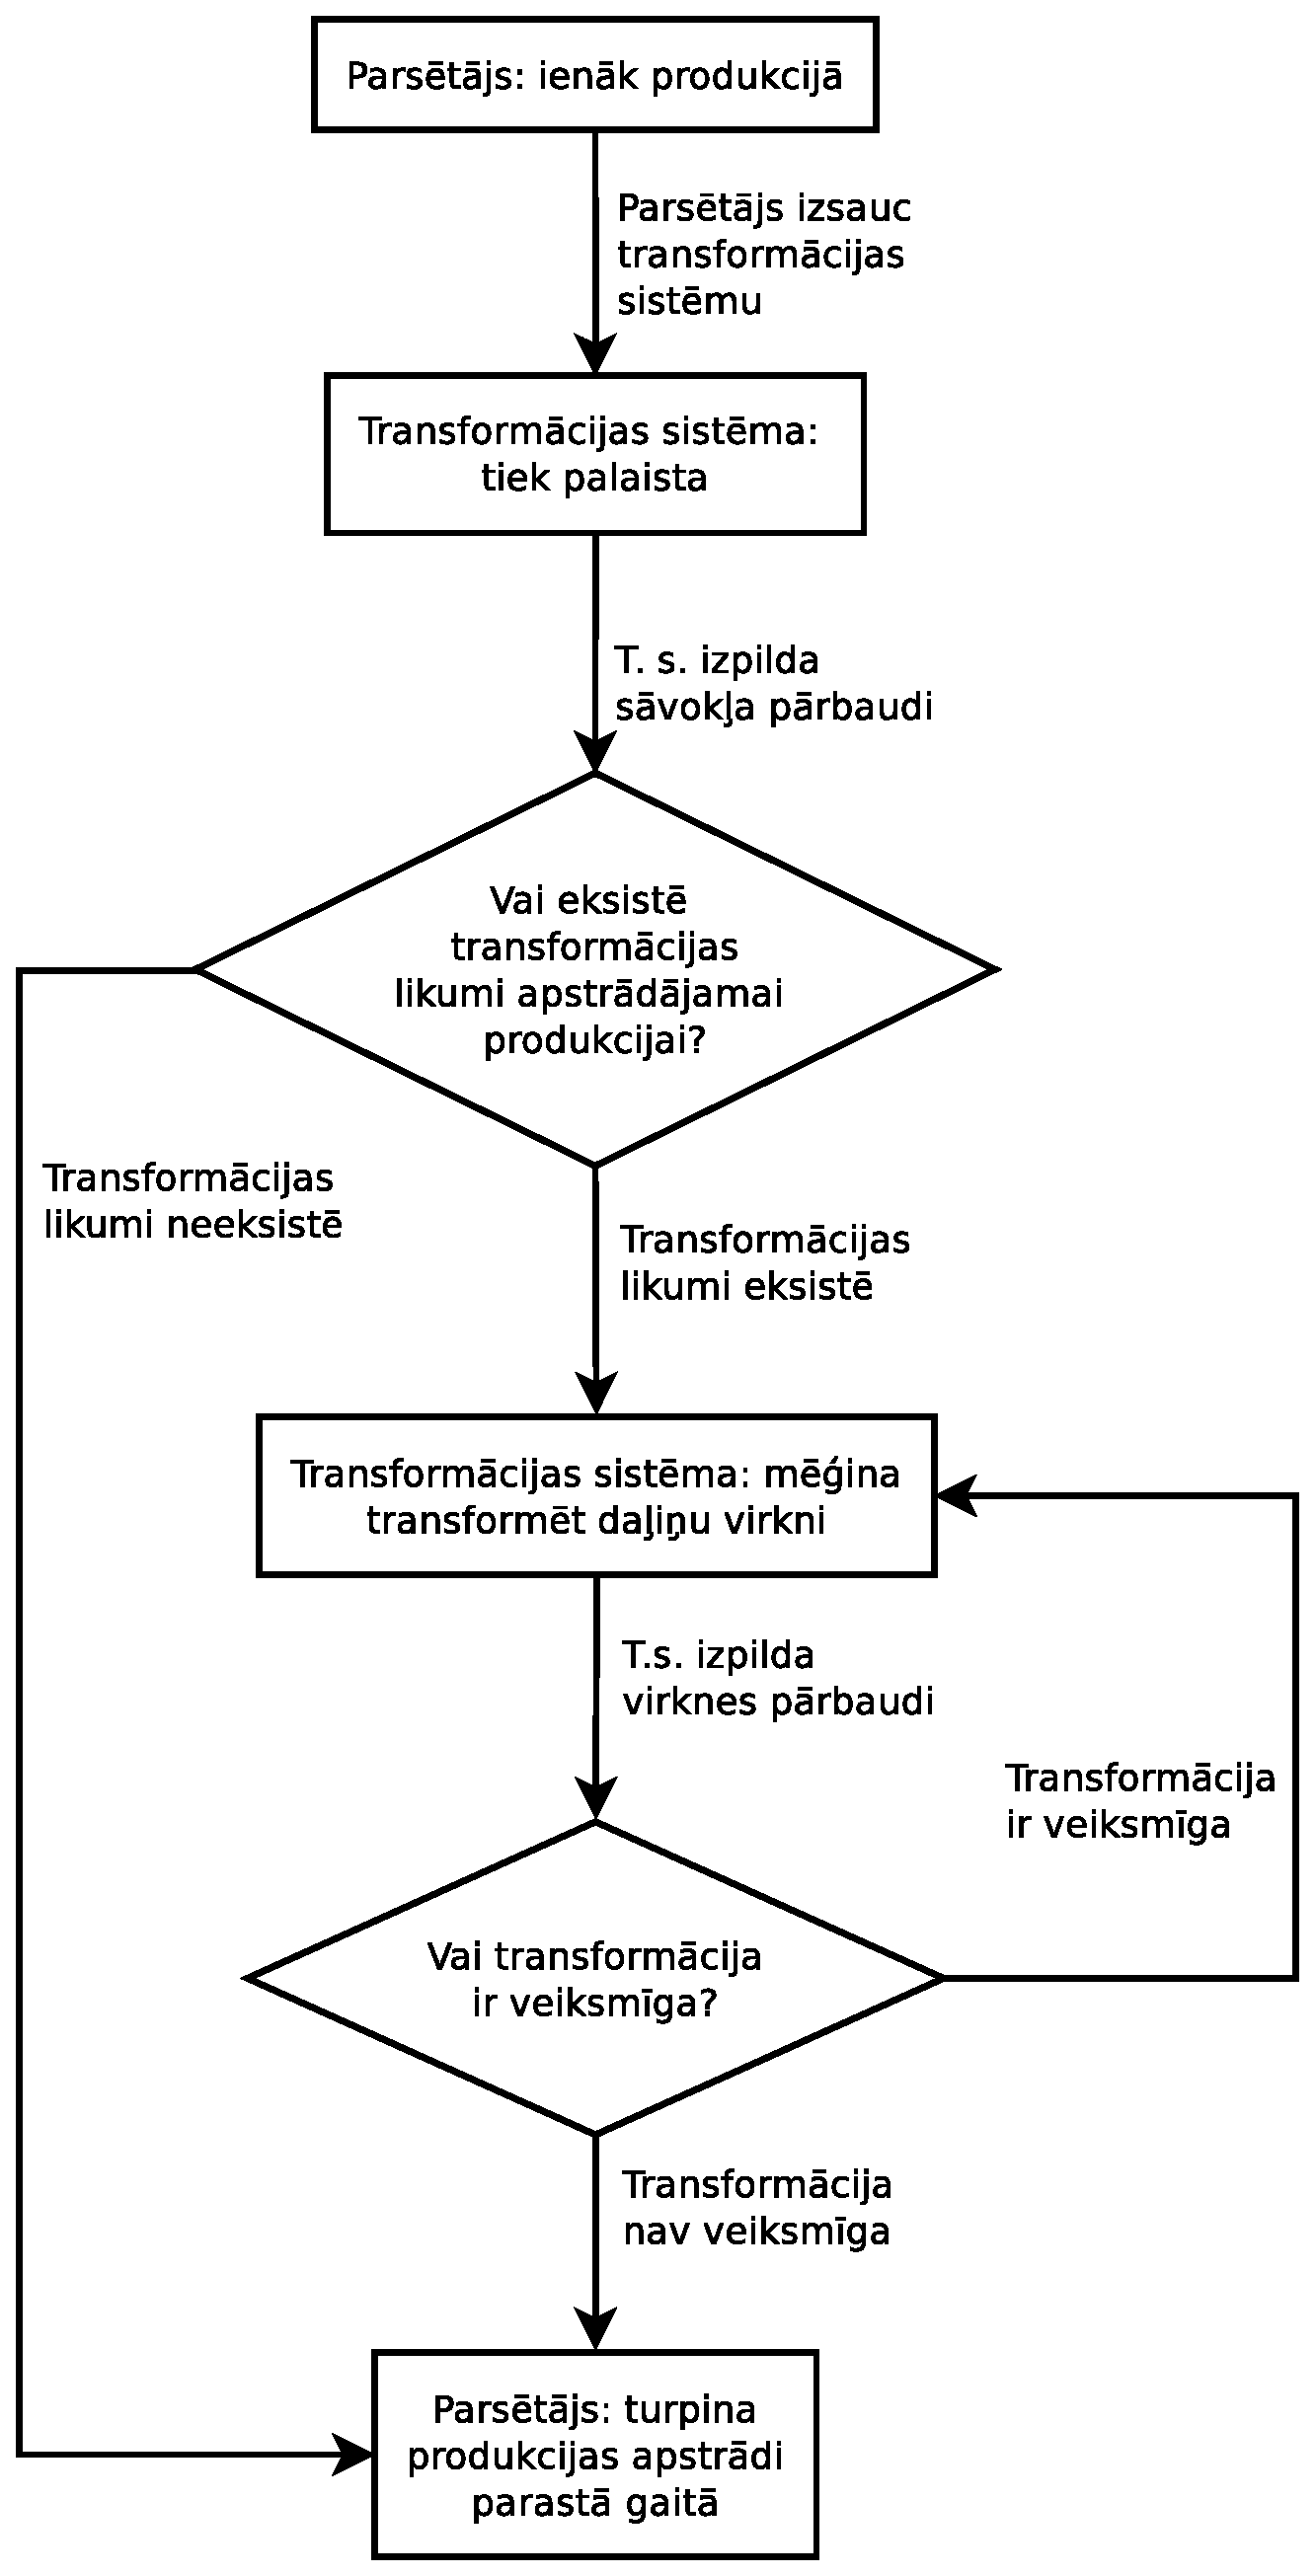
\includegraphics[scale=0.4]{pictures/match_algorithm}
  \caption{\label{fig:match_algorithm}Parsēšanas darba gaita ar iekļauto transformācijas sistēmu}
\end{figure}

\subsection{\label{sbs:sys_parserqualities}Parsētāju īpašības}

Šajā darbā piedāvātā sistēma tiek izstrādāta uz LL(k) parsētāja bāzes. Lai parsētājs varētu tikt integrēts ar aprakstāmo sistēmu, tam jābūt implementētam ar rekursīvas nokāpšanas algoritmiem LL(k) vai LL(*). LL parsētājs tika izvēlēts tāpēc, ka LL ir viena no intuitīvi saprotamākām parsētāju rakstīšanas pieejam, kas ar lejupejošo procesu apstrādā programmatūras tekstu. LL parsētājiem nav nepieciešams atsevišķs darbs parsēšanas tabulas izveidošanā, tātad parsēšanas process ir vairāk saprotams cilvēkam un vienkāršāk realizējams.

Tā kā transformāciju sistēma tiek veidota ka paplašinājums parsētājam, parsētājam jāatbilst dažiem nosacījumiem, kas ļaus sistēmai darboties. Zemāk ir aprakstītas īpašības, kuram jāpiemīt parsētājam, lai tas varētu veiksmīgi sadarboties ar aprakstāmo sistēmu.

\begin{description}
\item[Tokenu virkne]
Parsētājam jāprot aplūkot tokenu virkni ka abpusēji saistītu sarakstu, lai eksistētu iespēja to apstaigāt abos virzienos. Tam arī jādod iespēju aizvietot kaut kādu tokenu virkni ar jaunu un ļaut uzsākt apstrādi no patvaļīgas vietas tokenu virknē.

\item[Pseido-tokeni]
Parsētāji parasti pielieto (reducē) gramatikas likumus ielasot tokenus no ieejas virknes. Pseido-tokens, savukārt, konceptuāli ir atomārs ieejas plūsmas elements, bet īstenībā attēlo jau reducētu kaut kādu valodas gramatikas likumu. Viens no pseido-tokeniem, piemēram, ir tokens izteiksme - \verb|{expr}|, kas var sastāvēt no daudziem dažādiem tokeniem (piem. \verb|(a+b*c)+d|).

\item[Vadīšanas funkcijas]
Pirmkārt, mēs prasam, lai katra gramatikas produkcija tiktu reprezentēta ar vadīšanas funkciju (\emph{handle-function}). Ir svarīgi atzīmēt, ka šim funkcijām būs blakus efekti, tāpēc to izsaukšanas kārtība ir svarīga. Šīs funkcijas atkārto gramatikas struktūru, tas ir ja gramatikas produkcija A ir atkarīga no produkcijas B, A-vadīšanas funkcija izsauks B-vadīšanas funkciju. 

\item[Sakrišanas funkcijas]
Katras vadīšanas funkcijas darbības sākumā tiek izsaukta tā sauktā sakrišanas funkcija (\emph{match-function}). Sakrišanas funkcija ir transformācijas sistēmas saskarne ar signatūru \verb|(Parser, Production)| $\to$ \verb|Parser|. Tā pārbauda, vai tā vieta tokenu virknē, uz kuru rāda parsētājs, ir derīga kaut kādai transformācijai dotās produkcijas ietvaros. Ja pārbaude ir veiksmīga, funkcija izpilda sakrītošās virknes substitūciju ar jaunu virkni un parsētāja stāvoklī uzliek norādi uz aizvietotās virknes sākumu. Gadījumā,  ja pārbaude nav veiksmīga, funkcija nemaina parsētāja stāvokli, un parsētājs var turpināt darbu nemodificētas gramatikas ietvaros.
\end{description}

Ja izstrādājamās valodas parsētāja modelis atbilst aprakstītām īpašībām, tad tā var tikt veiksmīgi savienota ar aprakstāmo transformācijas sistēmu un ļaut programmētājam ieviest modifikācijas oriģinālās valodas sintaksē.

\subsection{\label{sbs:sys_macrosyntax}Makro sistēmas sintakse}

Makro izteiksmes strādā stingri kaut kādas produkcijas ietvaros, tāpēc makro sintaksē tiek lietoti tipi, kas tiek apzīmēti ar produkciju nosaukumiem. Tipi tiks lietoti lai nodrošinātu pseido-tokenu virknes korektumu sākotnējās gramatikas ietvaros pēc sintakses izmaiņu ieviešanas. Transformāciju sistēma sastāv no \emph{match} makro likumiem un transformāciju funkcijām. Makro kreisā puse satur regulāro izteiksmi no tokeniem un pseido-tokeniem, kas tālāk tiek izmantota lai atrast virkni, kurai šī transformācija ir pielietojama. Makro labā pusē ir atrodamas funkcijas, kas izpilda transformē tās tokenu virknes, kas tiek akceptētas ar makro kreisās puses šablonu.

Apskatīsim \textit{match} funkciju likumus, kas modificē apstrādājamās gramatikas produkcijas uzvedību. \emph{Match} makro sintakses vispārīgo formu var redzēt attēlā~\ref{fig:matchsyntax}.

\begin{figure}[h!]
\begin{verbatim}
match [\prod1] v = regexp → [\prod2] f(v)
\end{verbatim}
\caption{\label{fig:matchsyntax}\emph{Match} makro sintakses vispārīgā forma}
\end{figure}

Šīs apraksts ir uztverams sekojoši. Ja produkcijas \verb|prod1| sākumā ir atrodama pseido-tokenu virkne, kas atbilst regulārai izteiksmei \verb|regexp|, tad tai tiek piekārtots mainīgais ar vārdu \verb|v|. Mainīgais \verb|v| var tikt lietots makro labajā pusē kaut kādas funkcijas izpildē. Tātad ja tāda virkne \verb|v| eksistē, tā tiek aizstāta ar pseido-tokenu virkni, ko atgriezīs \verb|f(v)| un tālāk var tikt reducēta pēc gramatikas produkcijas \verb|prod2| likumiem. 

Regulārā izteiksme \verb|regexp| ir vienkārša standarta regulārā izteiksme, kuras gramatika ir definēta attēlā~\ref{fig:regexpsyntax}.

\begin{figure}[h!]
\begin{verbatim}
regexp          → concat-regexp | regexp
concat-regexp   → asterisk-regexp  concat-regexp
asterisk-regexp → unary-regexp * | unary-regexp
unary-regexp    → pseudo-token | ( regexp )
\end{verbatim}
\caption{\label{fig:regexpsyntax}Regulāro izteiksmju gramatika uz pseido-tokeniem}
\end{figure}

Pagaidām sistēmas prototipa izstrādē tiek lietota šāda minimāla sintakse, bet nepieciešamības gadījumā tā var tikt paplašināta.

Tagad mēs varam izveidot definētās makro sintakses korektu piemēru. Pieņemsim, ka ērtības dēļ programmētājs grib ieviest sekojošu notāciju absolūtās vērtības izrēķināšanai - \verb/|{expr}|/. Sākotnējā valodas gramatikā eksistē absolūtās vērtības funkcija izskatā \verb|abs({expr})|. Tad makro, kas parādīts attēlā~\ref{fig:matchsample1} izdarītu šo substitūciju, ļaujot programmētājam lietot ērtāku funkcijas pierakstu.

\begin{figure}[h!]
\begin{verbatim}
match [{expr}] v = {|} {expr} {|}
    → [{expr}] {id:abs} {(} {expr} {)}
\end{verbatim}
\caption{\label{fig:matchsample1}Makro piemērs \#1}
\end{figure}

Vēl viens korektā makro piemērs: pieņemsim, ka funkcija \verb|replace| ir definēta valodā $T$ ar trim argumentiem, un darba gaitā tā jebkurā pseido-tokenu virknē aizvieto elementus, kas sakrīt ar otro argumentu, ar trešo funkcijas argumentu. Pieņemsim arī, ka mums ir nepieciešams izsaukt funkciju \verb|bar| ar vienu argumentu, kas ir summa no funkcijas \verb|foo| argumentiem. Šādā gadījumā makro, kas parādīts attēlā~\ref{fig:matchsample2}, izpildīs nepieciešamu darbību.

\begin{figure}[h!]
\begin{verbatim}
match [{expr}] v = {id:foo} {(} {expr} ( {,} {expr} ) * {)}
    → [{expr}] {id:bar} (replace v {,} {+})
\end{verbatim}
\caption{\label{fig:matchsample2}Makro piemērs \#2}
\end{figure}

\subsection{\label{sbs:sys_qualities}Transformācijas sistēmas apakšsistēmas}

Šī nodaļa parāda sistēmas sadalīšanu uz trim neatkarīgam daļām. Pirmā no tām ir sakrišanu meklēšanas daļa. Tā tokenu virknē atrod makro šablonu satikšanas reizes. Otrā ir atrasto virkņu apstrādes daļa. Tā pārveido sakrišanas mehānisma atrasto tokenu virkni atbilstoši tam, kas norādīts makro labajā daļā. Trešā ir tipu pārbaudīšanas sistēma, kas statiski pārbauda, vai uzrakstītais makro var būt derīgs valodas gramatikas ietvaros. Šīs sadalījums ir tikai konceptuāls, kas ir izveidots ērtības dēļ, lai varētu apskatīt sistēmu ka atsevišķu apakšsistēmu kombināciju.

Šablonu sakrišanu meklēšanas sistēma ir īsumā aprakstīta apakšnodaļā~\ref{sbsbs:sys_matches}. Sīkāk šīs apakšsistēmas īpašības un tās prototipa realizācija ir aprakstīta nodaļā~\ref{s:prototype}.

Ir nepieciešams izveidot mehānismu, kas ļaus transformēt makro kreisās puses akceptētu pseido-tokenu virkni, izveidojot virkni, kas to aizvietos. Lai to izdarītu ir nepieciešama kaut kāds papildus rīks, par kuru ies runa apakšnodaļā~\ref{sbsbs:sys_language}.

Ir plānots, ka transformāciju sistēma varēs atpazīt nepareizi sastādītus makro šablonus lietojot tipu kontroli. Šīs pieejas bāzes principi ir aprakstīti apakšnodaļā~\ref{sbsbs:sys_typesystem}. Jāņem vērā tas, ka lai šī sistēma varētu tikt pielietota, izvēlētai transformāciju valodai jāpiemīt tipu secināšanas (\emph{type inference}) īpašībai.

\subsubsection{\label{sbsbs:sys_matches}Sakrišanu meklēšana}

\fixme{Uzrakstīt!}

\subsubsection{\label{sbsbs:sys_language}Tokenu virkņu apstrāde}

Gadījumā, ja šablonu sistēma nesaturētu regulāro izteiksmju sintaksi (it īpaši \verb|*|), būtu iespējams transformēt tokenu virknes ar pašu makro palīdzību. Atrastās tokenu virknes vienmēr būtu ar vienādu un determinētu garumu un saturu. Bet tā kā šabloni ļauj meklēt sakrišanas ar elementu sarakstiem, ir nepieciešams veids, kā apstrādāt jaunizveidotus un, iespējams, tukšus sarakstus.

Tātad lai varētu izpildīt atrastās tokenu virknes apstrādi un modificēšanu ir nepieciešams kaut kāds papildus rīks. Šīs rīks varētu būt kaut kāda programmēšanas valoda. Izplatītākās programmēšanas valodu paradigmas mūsdienās ir imperatīvā  vai funkcionālā paradigma. Katru no tiem varētu lietot atrasto virkņu apstrādei.

Šīm uzdevumam varētu lietot kādu no imperatīvam programmēšanas valodām, piemēram C, vienkārši izveidojot saskarni ar tās valodas kompilatoru. Bet vairākumam šādu valodu nav statiskas tipu secināšanas iespējas. Statiska tipu secināšana C valodas gadījumā ir neiespējama rādītāju mainīgo dēļ, kuru tipus nevar izrēķināt parsēšanas laikā. Lai varētu ieviest statiskās tipu izsecināšanas iespējas, vajadzēs ierobežot valodas iespējas, tātad modificēt eksistējošo kompilatoru vai kaut kā citādāk ierobežot pieejamo konstrukciju kopu.

Uzdevumam arī varētu lietot kādu no jau eksistējošām funkcionālām valodām ar tipu secināšanas īpašību. Tad nebūs nepieciešamības veidot savu valodu pilnīgi no jauna. Bet tas nozīmēs, ka būs rūpīgi jāizpēta izvēlētās valodas sintaksi, kas var būt pārāk grūti.

Varētu lietot arī vienu no jau eksistējošām funkcionālām valodām ar tipu secināšanas īpašību, kas piemīt vairākumam funkcionālo valodu.Vēl viena ērtā funkcionālo valodu īpašība ir tas, ka tās funkcijām nepiemīt blakusefekti, tātad to izpilde nevarēs samainīt eksistējošos datus. Valoda, kuras funkcijām ir blakusefekti, varētu sabojāta parsētāja darbu.

Šīs sistēmas implementācijā tika izvēlēts izveidot minimalistisku funkcionālu valodu, kura būs statiski tipizējama. Tātad visiem šīs valodas mainīgajiem varēs izsecināt piederību pie tipa un pie kaut kāda virstipa, kas tiks lietots lai nodrošināt transformāciju korektumu. Funkcionālā pieeja nodrošina arī to, ka apstrādes funkcijām nepiemīt blakusefekti, kas varētu samainīt eksistējošos datus. Valodas mērķis ir ļaut izveidot atrasto tokenu permutācijas ar kādiem papildinājumiem nepieciešamības gadījumā.

Galvenais šīs valodas pielietojums ir dot iespēju apstaigāt pseido-tokenu virkni, kura tika atzīta par sakrītošu ar atbilstošu šablonu. Lai to darīt, tā dos iespēju lietot rekursiju un dažas iebūvētās funkcijas - saraksta pirmā elementa funkciju \verb|head|, saraksta astes funkciju \verb|tail| un objektu pāra izveidošanas funkciju \verb|cons|. Funkcija \verb|cons| funkcionālo valodu kontekstā strādā kā saraksta izveidošanas funkcija, jo saraksts \verb|list(1, 2, 3)| tiek reprezentēta ka \verb|cons(1, cons(2, cons(3, nil)))|, kur \verb|nil| ir speciāls tukšs objekts. Valoda saturēs arī \verb|if| konstrukciju, kas ļaus pārbaudīt dažādus nosacījumus.

Lai būtu iespēja apstādināt rekursiju, šī valoda arī ļaus izpildīt aritmētiskās operācijas ar veseliem skaitļiem. Tas dos iespēju izveidot skaitītājus un izveidot rekursijas izejas nosacījumus.

Tiek plānots, ka šī valoda arī ļaus izpildīt daļēju novērtējumu izteiksmēm, tur kur būs nepieciešams. Tas nozīmē, ka valodai jāsatur saskarne, kas ļaus piekļūt pie tokena vērtības. Šim mērķim ir domāta funkcija \verb|value|, kas ir pielietojama pseido-tokeniem ar skaitlisku vērtību, piemēram, lai dabūt skaitli \verb|5| no pseido-tokena \verb|{int:5}|. Valoda arī ļaus izveidot jaunus tokenus ar izrēķinātu vērtību.

Funkcija \verb|type|, savukārt, ļaus pārbaudīt tokenu tipu, kas var būt nepieciešams transformācijas procesā, piemēram, lai atpazīt kādu operatoru.

Lai būtu iespēja apstādināt rekursiju, šī valoda arī ļaus izpildīt aritmētiskās operācijas ar veseliem skaitļiem. Tas dos iespēju izveidot skaitītājus un izveidot rekursijas izejas nosacījumus.

\subsubsection{\label{sbsbs:sys_typesystem}Tipu sistēma}

Kā bija redzams attēlā~\ref{fig:matchsyntax}, katrā makro pusē ir atrodams produkcijas nosaukums, \verb|[prod1]| un \verb|[prod2]|. Tas tiek darīts tādēļ, lai kontrolētu, kad dotais makro ir pārbaudīts, un kāda tipa izejas virkni tas radīs. Abas šīs atzīmes ir rādītas tipu kontroles sistēmas dēļ.

Katrs atsevišķs makro strādā konkrētas gramatikas produkcijas ietvaros, \verb|[prod1]| dotā makro gadījumā. Tas nodrošinās to, ka katrs no makro tiks izpildīts pareizajā vietā un visas konstrukcijas tiks apstrādātas. 

Otrais tips, \verb|[prod2]|, atzīmē to, ka pēc transformācijas procesa beigām mums jāsaņem tieši šādai produkcijai korektu izteiksmi. Tātad ir jāparbauda tas, ka funkcijas \verb|f(v)| rezultāts attiecībā uz atrasto tokenu virkni, ir atļauta ieejas virkne priekš produkcijas \verb|prod2|.

Lai to paveikt ir nepieciešams izveidot pseido-tokenu regulāro izteiksmi produkcijai \verb|prod2|. Tālāk ir nepieciešams izsecināt funkcijas \verb|f| no virknes \verb|v| rezultāta tipu.

Šajā darbā netiks apskatīts jautājums, kādā veidā tiks izveidota regulārā izteiksme priekš katras gramatikas produkcijas. To varētu izveidot programmētājs, vai, varbūt tā varētu tikt izveidota automātiski. Ir svarīgi pieminēt, ka pāreja no gramatikas likuma uz regulāro izteiksmi noved pie kādas informācijas zaudēšanas. Piemēram, nav iespējams uzkonstruēt precīzu regulāro izteiksmi valodai:

\begin{verbatim}
A :=  aAb | ab
\end{verbatim}

Tomēr ir iespējams izveidot regulāro izteiksmi kas iekļaus sevī gramatikas aprakstīto valodu, piemēram, \verb|a+b+|. Makro lietotā transformācijas shēma tiks atzīta par pareizo, ja ir iespējams pierādīt, ka produkciju aprakstošā regulārā izteiksme atpazīst arī valodu, ko veido \verb|f(v)|.

Ir viegli pamanīt, ka regulārās izteiksmes izveido dabisku tipu hierarhiju. Valoda, kura var tikt atpazīta ar regulāro izteiksmi $r_1$, var tikt iekļauta citas regulārās izteiksmes $r_2$ atpazītās valodā apakškopas veidā. Piemēram, regulārās izteiksmes \verb|a+| valoda ir atpazīstama arī ar regulāro izteiksmi \verb|a*|, bet \verb|a*| atpazīst vēl papildus tukšu simbolu virkni. Šādai tipu hierarhijai uz regulārām izteiksmēm eksistē arī super-tips, ko uzdod regulārā izteiksme \verb|.*| - $\top$. Ir acīmredzami, ka $\forall t_i \in R, t_i \sqsubseteq \top$, kur $R$ ir visu regulāro izteiksmju kopa.

Ir svarīgi izveidot procedūru, kas ļaus izsecināt, vai $r_1 {\sqsubseteq} r_2$. Ir zināms, ka ir iespējams katrai regulārai izteiksmei uzbūvēt minimālu akceptējošu galīgu determinētu automātu\footnote{Sk. nodaļu~\ref{sbs:prot_algorithms}.}. Šīs automāts atpazīs precīzi to pašu valodu, ko atpazīst regulārā izteiksme. Tas nozīmē, ka no $r_1 \sqsubseteq r_2 \Rightarrow seko min (det (r_1)) \sqsubseteq min (det (r_2))$. Diviem minimāliem automātiem $A_1$ un $A_2$, $A_1 \sqsubseteq A_2$ nozīmē, ka eksistē kaut kāds attēlojums $\Psi$ no $A_1$ stāvokļiem uz $A_2$ stāvokļiem, tāds, ka:

\[
    Start (A_1) \to Start (A_2) \in \Psi
\]
\[
    \forall s \in States (A_1) \forall e \in Edges (s),
    \Psi (Transition (s, e)) = Transition (\Psi (s), e)
\]

Šeit $States (x)$ apzīmē automāta $x$ stāvokļu kopu, $Edges (s)$ apzīmē pseido-tokenu kopu, kas atzīmē no stāvoļa $s$ izejošās šķautnes. $Transition(s, t)$, savukārt, apzīmē stāvokli, kas ir sasniedzams no $s$ pārejot pa šķautni, kas atzīmēta ar pseido-tokenu $t$.

Otra svarīga īpašība, kas tiks lietota šajā tipu pārbaudīšanas sistēmā ir tas, ka transformāciju valoda ir statiski tipizējama un tā satur ļoti ierobežotu iebūvēto funkciju skaitu. Katrai no šīm iebūvētām funkcijām ir iespējams izveidot to aprakstošo regulāro izteiksmi. Piemēram, regulārā izteiksme funkcijai $head (x)$ var tikt izveidota ka visu to šķautņu kopa, kas iziet no $x$ aprakstošā automāta sākuma stāvokļa. Kad šablona apstrāde tiek sākta, var arī izsecināt iespējamo virknes garumu intervālu un izvadīt brīdinājumus gadījumā, ja ir iespējama funkcijas $head (x)$ izsaukšana no tukšā saraksta.

Šī nodaļa tikai vispārīgi apraksta tipu secināšanas sistēmas ideju. Uz doto brīdi tā atrodas izstrādes stadijā, bet var redzēt ka tās izveide ir pamatota. Sīkāka informācija par tipu sistēmu ir saņemama pie Eq kompilatora izstrādes komandas.